\documentclass[10pt,twocolumn]{article}
\usepackage{array}
\usepackage[numbers,square,sort]{natbib}
\usepackage{multirow}
\usepackage{graphicx}
\usepackage[boxed]{algorithm2e}
\usepackage{breakurl}

\begin{document}

\title{Calculating Betweenness Centrality using CUDA}
\author{Gavin Gresham}
\maketitle

\section{Abstract}
The goal of this project is to create a CUDA \cite{cudaGuide} implementation of an algorithm to compute vertex betweenness centrality of social networking graphs. The benchmark being used is SNAP \cite{snapGraph}, a collection of social networking algorithms, including a CPU implementation of betweenness centrality. 
 
I use a modified version of the algorithm found in \cite{Brandes01afaster} to introduce parallelism at both the vertex level, as well as the neighbour detection level. This allows for a balance between both performance and memory usage. In this paper I will demonstrate the value of CUDA in the analysis of social network graphs, as well as discuss the current limitations of the technology.

\section{Problem}

\begin{algorithm}[HA]
%\SetLine
CB[v] $\leftarrow$, $v \in V$\;
\For{$s \in V$}
{
	S $\leftarrow$ empty stack\;
	P[w] $\leftarrow$ empty list, $w \in V$\;
	$\sigma [t] \leftarrow 0$, $t \in V$\; $\sigma [s] \leftarrow$ 1\;
	d[t] $\leftarrow - 1$, $t \in V$\; d[s] $\leftarrow$ 0\;
	Q $\leftarrow$ empty queue\;
	enqueue s $\rightarrow$ Q\;
	\While{Q not empty}
	{
		dequeue v $\leftarrow$ Q\;
		push v $\rightarrow$ S\;
		\For{neighbor w of v}
		{
			%\STATE
			\If{$d[w] < 0$}{
			
				enqueue w $\rightarrow$ Q\;
				$d[w] \leftarrow d[v] + 1$\;}
			
			\If{$d[w] = d[v] + 1$}{
			
				$\sigma[w] \leftarrow \sigma[w] + \sigma[v]$\;
				append v $\rightarrow$ P[w]\;
			}
		}	
	}


	$\sigma[v] \leftarrow 0$, $v \in V$\;
	\While{S not empty}
	{
		pop w $\leftarrow$ S\;
		\For{$v \in P[w]$}{$\delta[v] \leftarrow \delta[v] + \delta[v] / \delta[w] (1 + \delta[w])$\;}
		\If{$w \neq s$}{$CB[w] \leftarrow CB[w] + \delta[w]$\;}
	}
}

\caption{Brande's Algorithm}

\end{algorithm}
 
\section{Implementation}
I attempted three implementations of the betweenness centrality algorithm. First I will discuss the naive implementation which introduces parallelism to Brandes algorithm at the vertex level. It is straight forward to implement, but it has drawbacks, as I'll discuss. Next is the approach that adds parallelism to edge detection. This version is more complex and requires more attention to synchronization and memory conflicts. Finally there is a version that attempts to utilize additional GPUs with MPI. This version requires very few CUDA changes, but requires that memory be replicated across each GPU.
 
[Figure: Brandes Psuedo]
 
\subsection{Vertex Level Parallelsim}
With very little modification, we can add parallelization to Brandes algorithm. The outer loop, that iterates through each vertex in the graph, operates independently of previous and future iterations. This CUDA implementation assigns a thread to each vertex in the graph.
 
There are several benefits to this approach. It is straight foward and easy to understand. You could implement the same code on CPU architectures without complications.
 
However, drawbacks exist as well. Brandes algorithm conserves space when executed sequentially, but when run in parallel any array that is mutable has to be copied to every parallel thread. The only memory that is shared is the cummulative betweenness centrality score and the array of edges. This leads to an exponential growth in memory as the number of vertices rises. The overall memory usage ends up being $|V| * (5|V| + |E|)$, which quickly becomes impractical above graphs with vertices numbering for than 4000.
 
\subsection{Edge Discovery Parallelism}
\label{implBFS}
This implementation is intended to utilizes CUDA's high amount of low powered threads while optimizing for its memory restrictions. The basis of the algorithm is still based on \cite{Brandes01afaster}, but has several modifications to ease thread synchronization and memory access penalties.
 
The algorithm is aware of the properties of a CUDA warp. In the current hardware generation, 32 threads operate simultaneously on instructions and are able to combine adjecent memory reads and writes to a single operation. Given the latency for accessing global memory, this is a crucial feature to exploit. When a warp reaches the section of code that requests the next set of vertices from the frontier queue, 32 vertex indices are popped from the queue for a more efficient transaction. Under ideal circumstances it will be done in 4 memory reads, though if the queue elements are not 32 byte aligned it could be 5 reads. The same method is used after all the shortest paths are found to retrieve batches of vertex indices from the stack.
 
Unfortunately, the same opportunities for memory optimizations do not exist in other sections of the code. The nature of social networking graphs means that a vertex could be connected to any other vertex in the graph, which makes sequential reads during the edge discovery phase improbable. Additionally, the fact that each vertex will have a variably edge degree means that CUDA warps will diverge. Under normal operations every thread in a warp executes an instruction simultaneously. When one or more threads diverge instructions must now be run sequentially until the threads once again converge.
 
An area that will have less reliable memory optimization is writing to the predecessor list. These are stored in linked list structure where the first $|V|$ array slots correspond to the first predecessor found for the vertex with index $ \in V$ and array slots $|V|$ through $|E|$ are empty space for any linked list to expand into. A pointer in shared memory exists to the next empty slot in the array and is initialized to $|V|$, the first element of the expansions section. When a thread needs to add a new node to a vertex's linked list the pointer must be updated atomically. In an idea situation, all warp threads will need to expand a linked list and the $atomicAdd()$ function will return sequential indices. This would result in a very efficient global write. However, it is possible that another warp will be requesting a pointer for free space at the same moment, and the indices could be distributed among the competing warps. While some memory could still be coalesced and stored using reduced instruction, optimal throughput will not be achieved. There seems to be no way to allow a warp exclusive access to an atomic variable without causing a significant delay to running time.

\subsection{MPI Enhanced}
Expanding upon the work described in the previous section, support for platforms with multiple GPUs and high performance computing clusters was added. The CUDA code was modified to compute designated segments of vertices allowing the work to be distributed amongst a variable number of network nodes. It is important to note that the memory requirement for each GPU is still the same as the implementation discuseed in Section \ref{implBFS}. This means that an MPI solution will not be able to compute betweenness centrality on any arbitrarily large graph, but lowering the number of vertices a GPU computes in parallel in direct correlation to the number of added GPUs could allow for large graphs to be computed without reducing overall throughput.

The actual addition of MPI is fairly simple. All that is needed is the number of processes and the rank fo the current MPI node. Each node calls CUDA with this information as parameters. From this information, the method knows how large each block of vertices is and which block it's responsible for. This block can be futher divided on the MPI node depending on how many GPUs are present. Once all CUDA processes are finished there is an $MPI\_Reduce$ to sum the arrays of betweenness centrality computed on each node.

All multi-GPU test runs were performed on Jinx using 2 nodes for a total of 4 GPUs.

\section{Results}

\begin{table*}[h]
\centering
\label{tbl:compare}
\begin{tabular}{|c|c|c|c|c|c|c|c|}
\hline
\multirow{2}{*}{Elements*}& \multicolumn{4}{c|}{Running Time ($\mu sec$)} & \multicolumn{3}{c|}{Speedup relative to SNAP}\\\cline{2-8}
&SNAP&Vertex**&Edge Discovery&MPI&Vertex&Edge Discovery&MPI\\\hline
32 & 6578 & 2761 & 621 &  & 0.4197 & 4.4460 & \\\hline
64 & 18334 & 3141 & 751 &  & 0.1713 & 4.1824 & \\\hline
128 & 63658 & 4726 & 1563 &  & 0.0742 & 3.0236 & \\\hline
256 & 235117 & 11001 & 4637 &  & 0.0467 & 2.3724 & \\\hline
512 & 877849 & 36408 & 17614 &  & 0.0414 & 2.0669 & \\\hline
1024 & 3488531 & 144980 & 75415 &  & 0.0415 & 1.9224 & \\\hline
2048 & 14091411 & 613503 & 325096 & 4990026 & 0.0435 & 1.8871 & 0.1229\\\hline
4096 & 58778463 & 2444659 & 1379843 & 5262252 & 0.0415 & 1.7716 & 0.4645\\\hline
8192 &  & 7809208 & 5743033 & 6391250 &  & 1.3597707 & 1.2218\\\hline
16384 &  & 31269805 & 23653931 & 11000316 &  & 1.3219 & 2.8426\\\hline
32768 &  & 135979049 & 96906222 & 29873519 &  & 1.4032 & 4.5518\\\hline
65536 &  & 697781059 & 394990289 & 106874874 &  & 1.7665 & 6.5289\\\hline
131072 &  & 2490728678 & 1603625399 & 415907759 &  & 1.5531 & 5.9886\\\hline
\end{tabular}
\caption{The running time of each CUDA implementation and speedup relative to SNAP based on the size of the input graph.\newline
{\scriptsize *$|E| = 4|V|$ \newline
** Vertex Parallelism could not be performed on graphs where $|V|>4096$ due to memory constraints.}
}
\end{table*}

\subsection{Vertex Level Parallelism}
This simple parellization of Brandes algorithm has very poor performance compared to SNAP. It runs at about 5\% of the FLOPS that SNAP can operate at as seen in Table \ref{tbl:compare}. Additionally, it can't run on input files with more than 4096 vertices due to memory requirements.

One of the key problems is CUDA thread occupancy. Without additional threads per vertex some resources on the GPU are left idle. CUDA operates best when you can achieve a high occupancy with warps operating on similar tasks. A naive implementation of Brandes algorith simply has too much divergence.

Memory locality is also not considered in vertex level parallelism. Each vertex maintains its own data structures for the frontier, predecessor list, path count, and found vertex stack. These exist in one large array in global memory and threads in a warp will rarely, if ever, access sequential memory locations.

\subsection{Edge Discovery Parallelism}
Being optimized for CUDA, this implementation beformed significantly better than vertex level parallelism. As seen in Table \ref{tbl:compare} as the graph size increases the speedup in relation to SNAP plateaus at around 1.5x. These results are due to tuning parameters to work with the m2050/m2070 devices that are used on the Jinx cluster \cite{jinx}. Running this algorith on another device would likely require adjusting the number of threads per vertex, as well as the maximum number of vertices that are being processed at any one time.

\begin{figure}[htbp]
\centering
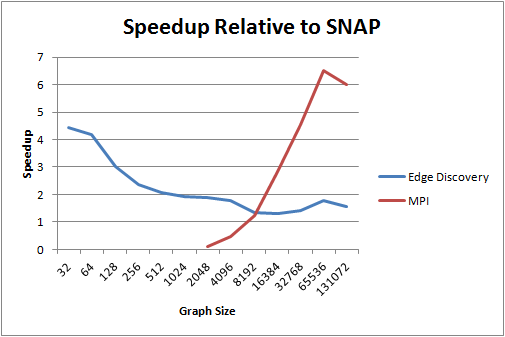
\includegraphics[scale=.6]{speedup.png}
\caption{The speedup of the Edge Discovery and MPI implementations in relation to SNAP as a function of graph size.}
\label{fig:speedup}
\end{figure}

\subsection{MPI Enhanced}
Combined with the changes from section \ref{implBFS} the MPI implementation shows the greatest speedup by far. It adds near linear speedup compared to the edge discovery parallelism that directly correlates to the number of GPUs used. An exception to this is when the segments of vertices assigned to a GPU is so small that the overhead of running MPI and CUDA memory allocation represent a significant percentage of the running time. It can be seen from Fig. \ref{fig:speedup} that the optimal time to use a configuration with 4 GPUs would be after $|V| > 8192$.

\section{Future Work}
Currently the usage of shared memory is limited to tracking the graph frontier and the state of the stack and queue. This leaves much of the shared memory unused despite the fact that it has a significantly lower access time than global memory. Any array that could be stored in shared memory quickly outgrows the 48KB available to CUDA 2.0 devices and I have thought of no other use for it.

Automatic parameter optimization

Snap integration

\bibliography{Bibliography}
\bibliographystyle{plainnat}
\end{document}
